\documentclass{article}

% 导入宏包
\usepackage{fancyhdr}
\usepackage{ctex}
\usepackage{listings}
\usepackage{graphicx}
\usepackage[a4paper, body={18cm,22cm}]{geometry}
\usepackage{amsmath,amsthm,amssymb,amstext,wasysym,enumerate,graphicx}
\usepackage{float,abstract,booktabs,indentfirst,amsmath}
\usepackage{array}
\usepackage{multirow}
\usepackage{url}
\usepackage{diagbox}
\usepackage{enumitem}
\usepackage{xcolor}
\usepackage{makecell}
\usepackage{tikz}
\usepackage{tcolorbox}
\usetikzlibrary{positioning, arrows.meta, automata}
\usepackage[bookmarks=true, colorlinks, citecolor=blue, linkcolor=black]{hyperref}


% 设置段落
\renewcommand\arraystretch{1.4}
\setlength{\parindent}{2em}
\setCJKmonofont{黑体}

% 设置高亮文字
\newtcbox{\mybox}[1][red]
{on line, arc = 0pt, outer arc = 0pt,
	colback = #1!10!white, colframe = #1!50!black,
	boxsep = 0pt, left = 1pt, right = 1pt, top = 2pt, bottom = 2pt,
	boxrule = 0pt, bottomrule = 1pt, toprule = 1pt}

% 配置代码显示
\lstset{
	xleftmargin = 3em,
	xrightmargin = 3em,
	aboveskip = 1em,
	backgroundcolor = \color{white},
	basicstyle = \small\ttfamily,
	rulesepcolor = \color{gray},
	breaklines = true,
	numbers = left,
	numberstyle = \small,
	numbersep = -14pt,
	keywordstyle = \color{purple}\bfseries,
	commentstyle = \color{green!60!black}, % 修改注释颜色
	stringstyle = \color{red!60!green!90!blue!90},
	morekeywords = {ASSERT, int64_t, uint32_t},
	moreemph = {ASSERT, NULL},
	emphstyle = \color{red}\bfseries,
	moreemph = [2]{int64\_t, uint32\_t, tid\_t, uint8\_t, int16\_t, uint16\_t, int32\_t, size\_t, bool},
	emphstyle = [2]\color{purple}\bfseries,
	frame = shadowbox,
	showspaces = false,
	columns = fixed
	morecomment = [l][\color{green!60!black}]{+}, % 设置以+开头的代码行为绿色
}

%--------------------页眉--------------------%

\pagestyle{fancy}
\fancyhead[L]{}
\fancyhead[R]{}
\fancyhead[C]{华东师范大学软件工程学院作业}
\fancyfoot[C]{-\thepage-}
\renewcommand{\headrulewidth}{1.5pt}

%--------------------标题--------------------%

\begin{document}
	
	\begin{center}
		{\Large{\textbf{\heiti 软件工程学院形式语言与自动机理论作业}}}
		\begin{table}[htb]
			\flushleft
			\begin{tabular}{p{0.4\linewidth}p{0.27\linewidth}p{0.28\linewidth}}\\
				\textbf{实验课程}:形式语言与自动机理论  & \textbf{年级}:2023级       & \textbf{姓名}:顾翌炜  \\
				\textbf{实验编号}:ch-2-4    & \textbf{学号}:10235101527 & \textbf{作业日期}:2025/03/25  \\
			\end{tabular}
		\end{table}
	\end{center}
	\rule{\textwidth}{2pt}
	
	\section*{课后作业}
	
	Convert the foilowing DFA to RE using state elimination technique
	
	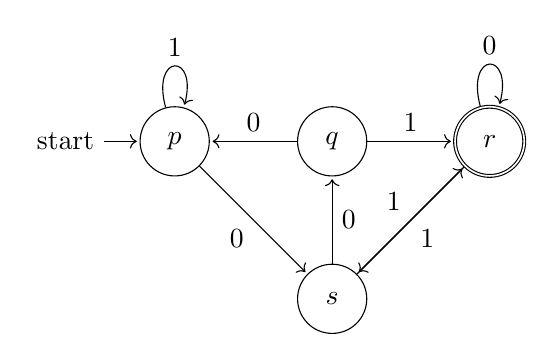
\begin{tikzpicture}[shorten >=1pt, node distance=2cm, on grid, auto]
		\node[state, initial] (p) {$p$};
		\node[state] (q) [right=of p] {$q$};
		\node[state] (r) [right=of q, accepting] {$r$};
		\node[state] (s) [below=of q] {$s$};
		
		\path[->]
		(p) edge [loop above] node {1} ()
		edge [swap] node {0} (s)
		(q) edge [swap] node {0} (p)
		edge node {1} (r)
		(r) edge [loop above] node {0} ()
		edge [swap] node {1} (s)
		(s) edge [swap] node {0} (q)
		edge [swap] node {1} (r);
	\end{tikzpicture}
	
	\section*{解答}
	
	\begin{figure}[H]
		\centering
		\includegraphics[width=11cm,angle=270]{./images/answer.jpg}
		\caption{answer}
	\end{figure}
	
\end{document}
